%% The following is a directive for TeXShop to indicate the main file
%%!TEX root = Thesis_Driver.tex
\graphicspath{{./Figures/}}
\chapter{Equivalent Magnetized Source}
\label{ch:Chap5_Equivalent_Source}

\section{Magnetic Data Processing}
As introduced in equation \ref{LinFowardAmp}, Magnetic Amplitude Inversion (MAI) makes use of amplitude data  with weak dependency on the magnetization direction in order to extract structural information. There is to date no instrument that can directly measure amplitude data. Amplitude data must therefore be derived from three-components magnetic field data such that:
\begin{equation}\label{AmpMagData}
\mathbf{|B|} = 
	\begin{bmatrix}
		\mathbf{B_x}^2 + \mathbf{B_y}^2 + \mathbf{B_z}^2
	\end{bmatrix} ^{1/2} 
\end{equation}
While there has been recent advancement in instrumentation measuring three-component field data, the vast majority of current and past airborne magnetic surveys consist of Total Magnetic Intensity (TMI) measurements.  Moreover, large uncertainties associated with the location and orientation of three-components data limit its use. 
Much efforts have been invested in extracting vector components data directly from TMI mearuements, either in the frequency domain or by an equivalent source technique. 

The method use frequency filtering has dominated the litterature since the early in 1960, giving rise to a swath of signal processing tools such as interpolation, upward continuation, filtering and derivative calculations.  
As demonstrated by \cite{Bhattacharyya64}, magnetic field anomalie (TMA) measurements can be expressed in cartesian coordinates as 2D Fourier-series expansion of the form:
\begin{equation}\label{TMA_Harmonic}
\begin{split}
TMA(x,y,z) = \sum_{n=o}^\infty  \sum_{m=o}^\infty \; & e^{{ -2 \pi \; z \; \Big( \frac{m^2}{{L_x}^2} + \frac{n^2}{{L_y}^2} \Big) }^{1/2}} \\
& \Big(A_m \cos{2\pi m \frac{x}{L_x}} + B_m \sin{2\pi m \frac{x}{L_x}}\Big) \\
& \Big(C_m \cos{2\pi n \frac{y}{L_y}} + D_m \sin{2\pi n \frac{y}{L_y}}\Big)
\end{split}
\end{equation}
where $ L_x$ and $L_y$ are the fundamental wavelengths in the $x$ and $y$ directions. The coefficients $A_m$, $B_m$, $C_n$ and $D_n$ are computed from the data for each wavenumbers $m$ and $n$. The harmonic representation of the data in \eqref{TMA_Harmonic} can be seen as a product of two functions: an exponential function controling the amplitude of the signal and an harmonic function for the spatial distribution. Converting data from the spatial domain to the wavenumber domain requires two important assumptions: that the data is located on a plane and distributed over a uniform grid. In most cases, airborne magnetic surveys are collected along flight lines widely spaced and flown over uneven topography, which makes the transformation unpractical.
The method of Taylor's Series approximation can be used to interpolate the data over a grid. This method become problematic however near regions with overlapping data collected at different elevation. In 2D, the rapid change in value requires high-order polynomial terms, which introduces unwanted structure in the gridded data.
 
The equivalent source method  has been suggested as an alternative to horizontal gridding methods \cite[]{Dampney69}. The technique makes use of the inherent ambiguity in determining the source of gravity field measurments. It can be shown that any magnetic response can be explained by an arbitrary distribution of sources. In discrete form, this problem gives rise to an underdetermine system of equations relating the equivalent surface to the data
\begin{equation}\label{ES_LeastSquare}
	\mathbf{F\;m = d}
\end{equation}
 an equivalent source is found by solving a least-squares problem:
\begin{equation}\label{ES_LeastSquare}
	\underset{m}{\text{min}} \| \mathbf{F\;m - d}\|_2
\end{equation}
As demonstrated by \cite{Dampney69}, the distance between the data and the equivalent source is limited by the frequency content of the signal.

The wavelet-domain formulation of \cite{LiOldenburg10} show that the equivalent source method can be done efficiently.
Most recent work by \cite{LiNabighian14} addresses striation artefacts when applying a reduction to the pole at low-latitude. They advocate for a positivity constraint formulation and prove the existance of such all-positive equivalent sourve layer in the 2D Fourier domain.
I here replicate the synthetic example presented in their study and shown in \ref{fig:ES_Li_True}. 
The model consists of a 200 unit cubes with susceptibility of 0.01 SI placed in a nonsusceptible model. Data is generate on a plane exactly 1 unit above the anomaly, assuming a purely vertical inducing field of 35,000 nT. Random Gaussian noise with standard deviation of 1 nT is added to the components of fields, from which TMI and amplitude data are calculated.
Using \cite{LiNabighian14} formulation, we then procede with an equivalent source inversion with positivity constraint. 
The equivalent source layer is placed at a depth that is half the data spacing, in this case at half a unit below the data plane.
Figure \ref{fig:ES_Li_Full_Space} presents the equivalent source layer, as well as the residual between the observed and predicted data. 
All three components of the field, and consequently the amplitude data $\mathbf{|B|}$, are well recovered within the noise level. 

\subsection{Complications}
Numerical experimentations show that the procedure proposed by \cite{LiNabighian14} breaks down in cases where the signal present in the data does not decays near the edges of the dataset. 
This type of situation is fairly common in mineral exploration as airborn surveys are flown along fix grids, regardless of regional and local magnetic anomalies. 
I illustrate this case with the same synthetic anomaly, but this time aftee removing a corner of data over the anomalie. 
Using the same parameter, I compute a new equivalent source layer as shown in figure \ref{fig:ES_li_CornerOut}.  
Unexpected anomalies appear in the $\hat x$ and  $\hat y$ components of the field along the North-West limit of the data. 
Although this edges artefact does not show in the TMI data, it has an important impact on the recovered amplitude data, resulting in a 
sizeable 50 nT anomaly, within the range of the true data.
Inverting such dataset would result in fictictious a distorted effective susceptibility model.
Similar issues arise at low-latitude it magnetic fields stretching along the declinaison of the inducing field.
There had been no studies to date looking into the stability of equivalent source methods to accurately recover all three components of the magnetic field.
This simple test seems to show that the distrubtion of equivalent sources near the edge of the survey is important. 
The following section proposes a solution via an equivalent magnetized source (EMS) layer.
  
\begin{figure}[h!]
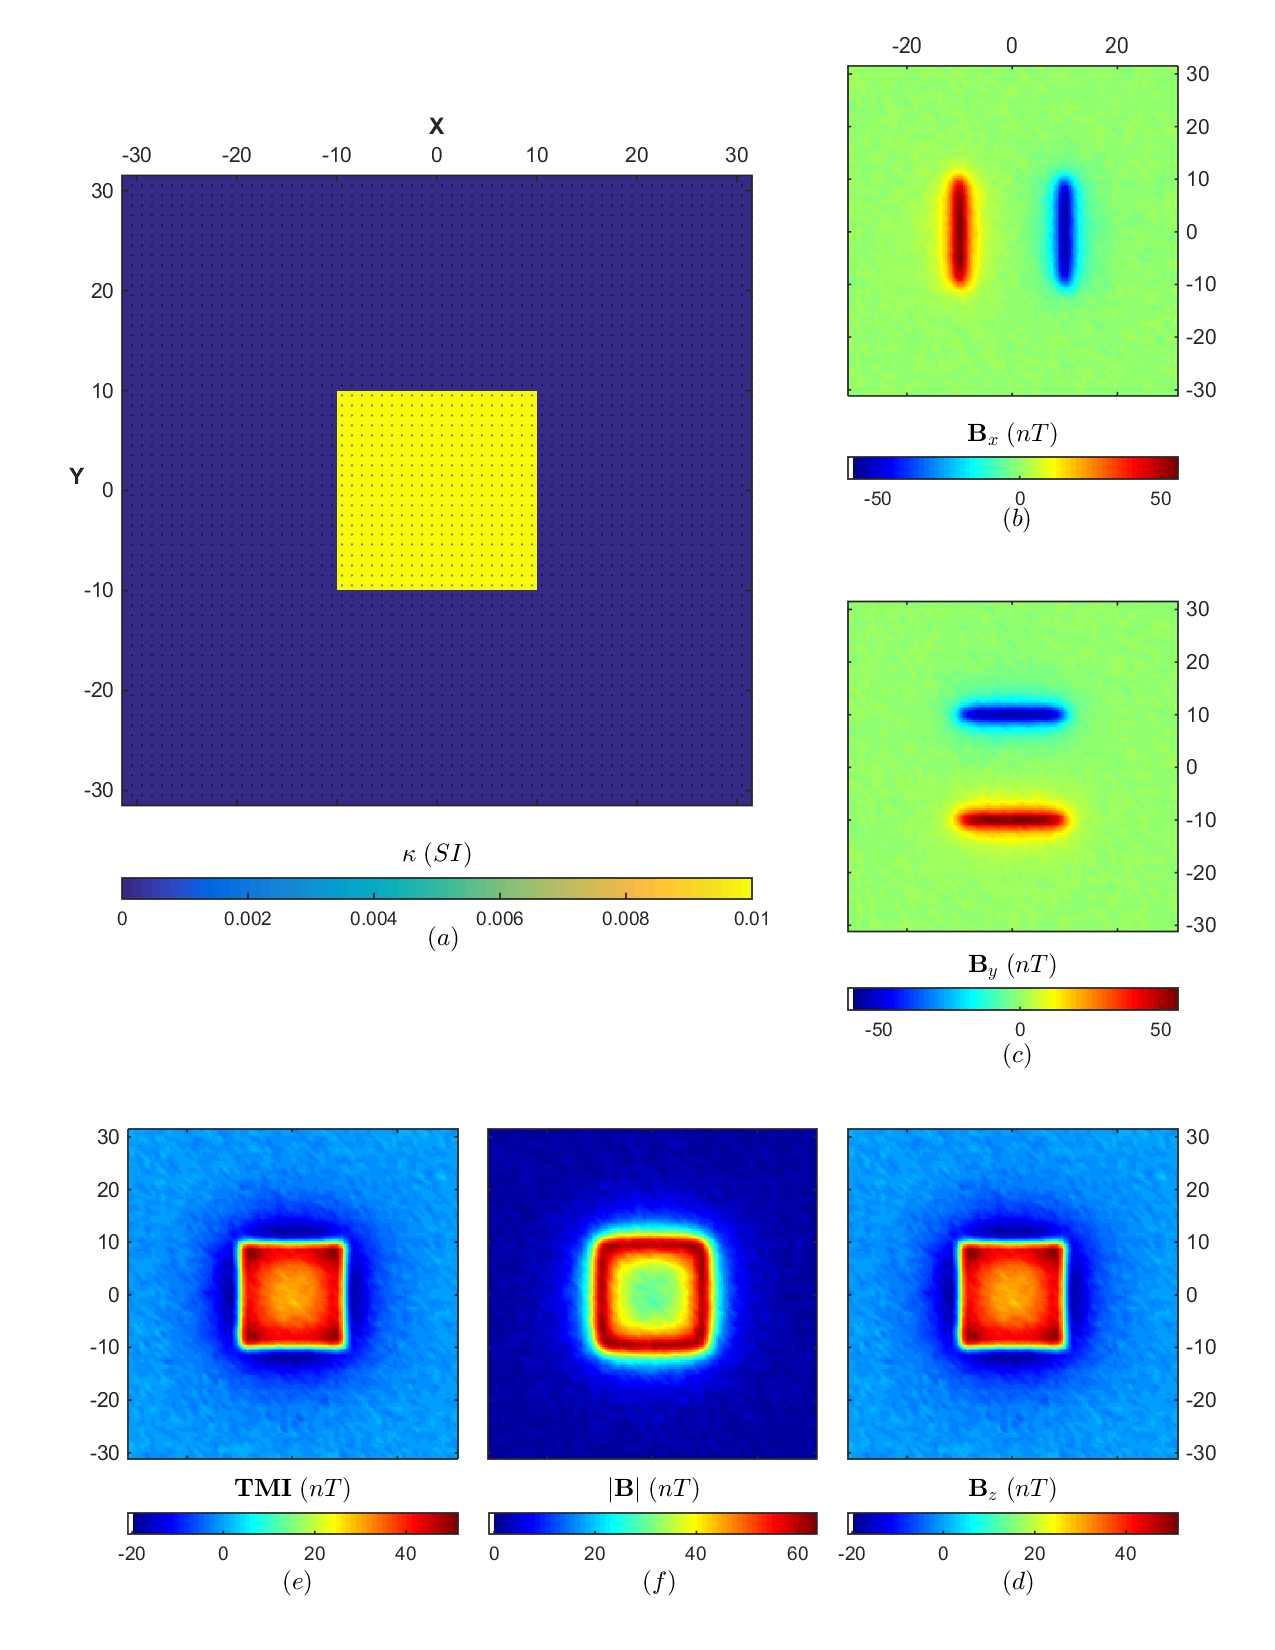
\includegraphics[scale=0.60]{ES_Li_True}
\caption{(a) Synthetic model consisting of a $200$ unit cubes of susceptible material in a nonsusceptible background. Data are generate on a plane one unit above the source location, assuming a purely vertical inducing field. Various components of the fields are shown in figure (b) to (f). }
\label{fig:ES_Li_True}
\end{figure}

\begin{figure}[h!]
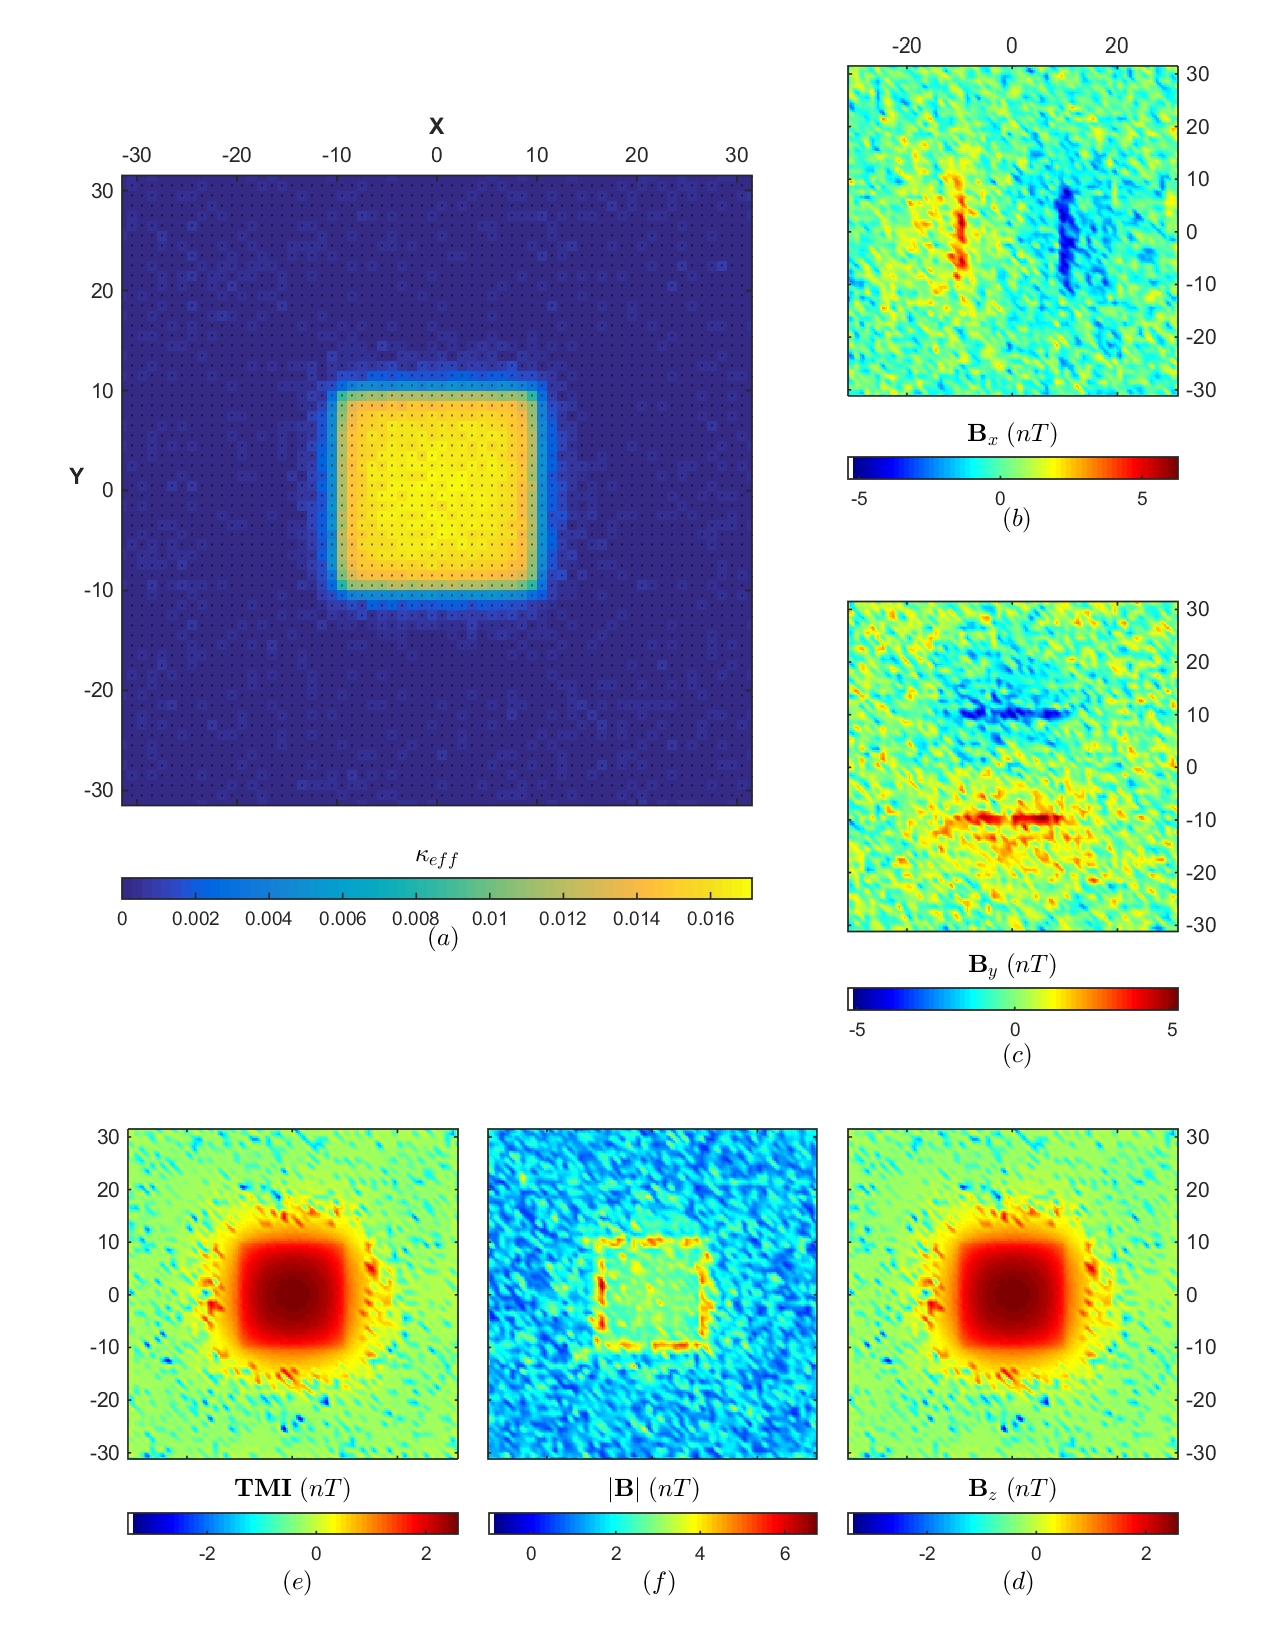
\includegraphics[scale=0.60]{ES_Li_Full_Space}
\caption{(a) Recovered equivalent source layer from TMI data using positivity contraint. The residual between observed and predicted data are shown in figure (b) to (f) for various components of the field. Each component is well recovered within the noise level.}
\label{fig:ES_Li_Full_Space}
\end{figure}

\begin{figure}[h!]
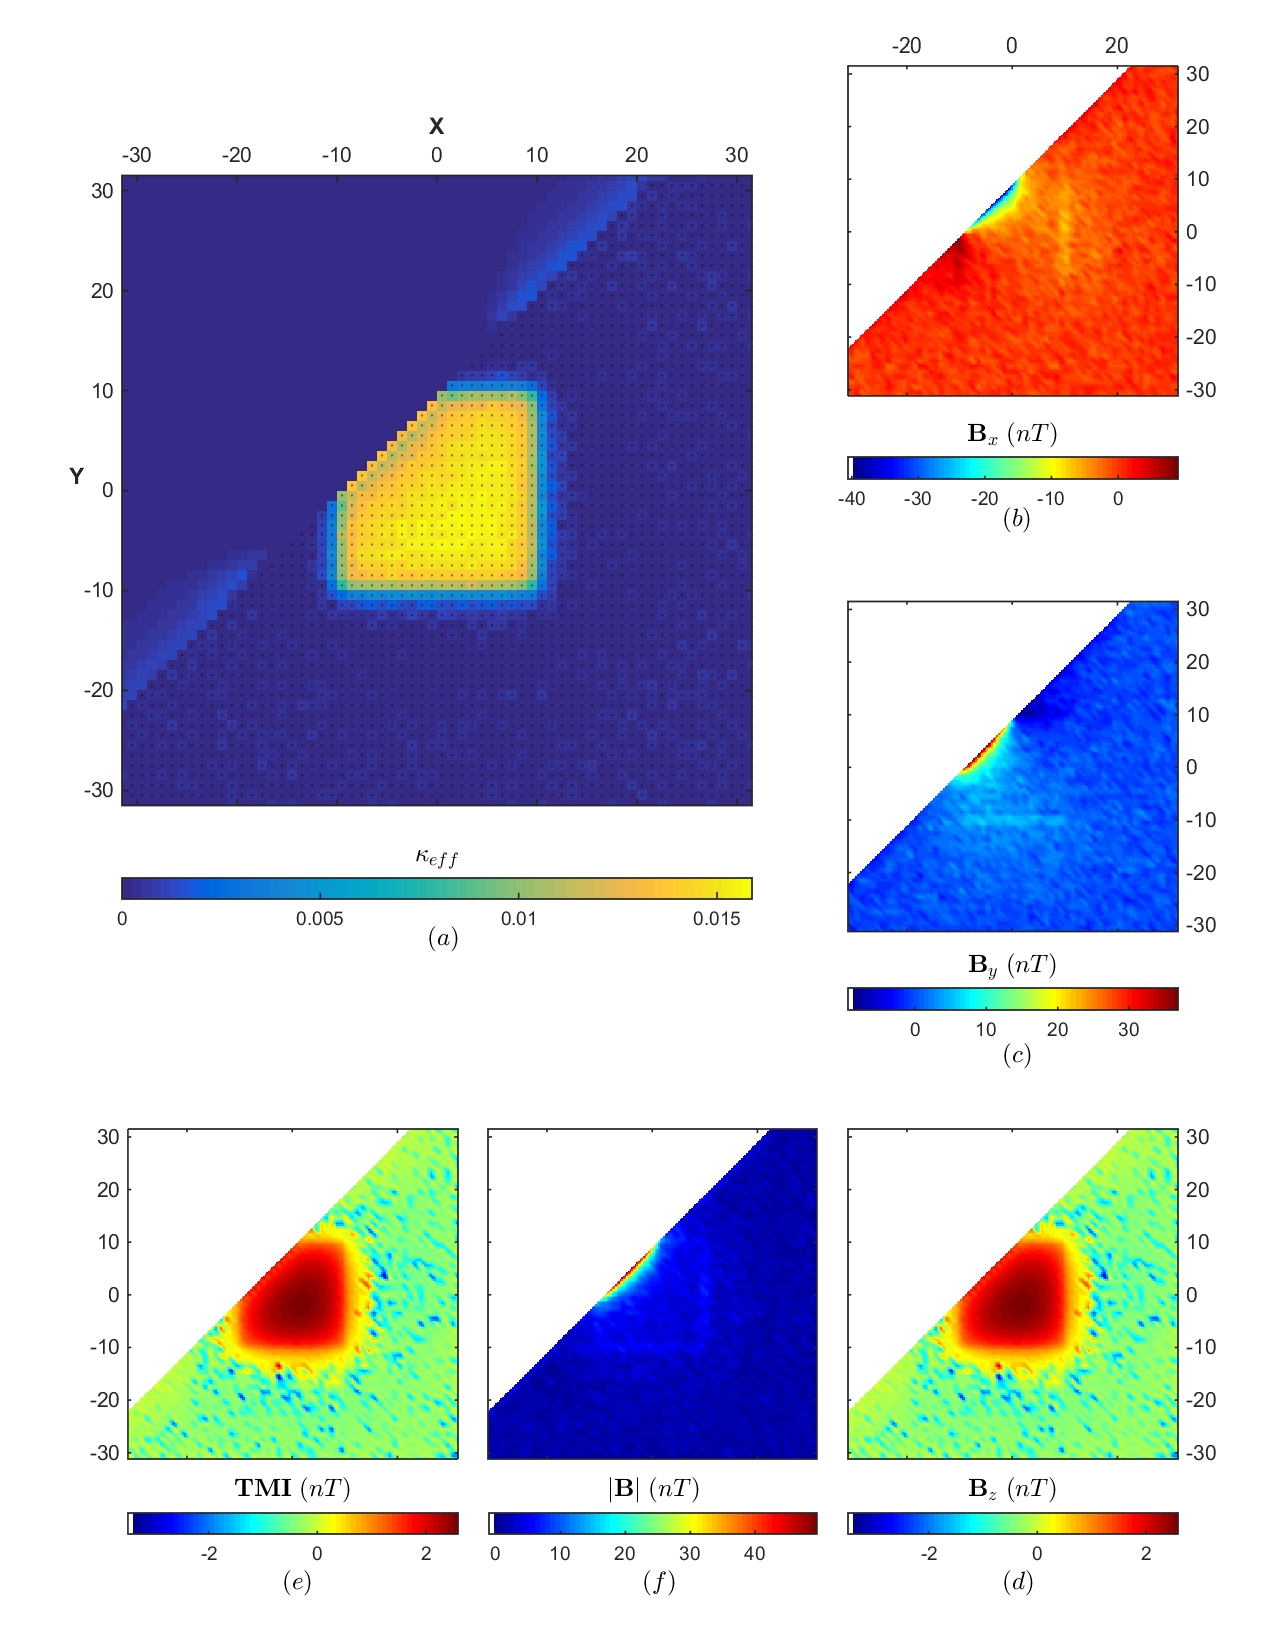
\includegraphics[scale=0.60]{ES_Li_CornerOut}
\caption{(a) Recovered equivalent source layer with positivity contraint on a subset of the original TMI data. The residual between observed and predicted data are shown in figure (b) to (f) for various components of the field. Additional structure appears in the predicted data as coherent noise in the $\hat x$ and  $\hat y$ components of the field, which are orthogonal to the inducing field oriented in $\hat z$. The TMI data is well recovered, but large errors are introduced in the amplitude data $\mathbf{|B|}$ }
\label{fig:ES_Li_CornerOut}
\end{figure}

\begin{figure}[h!]
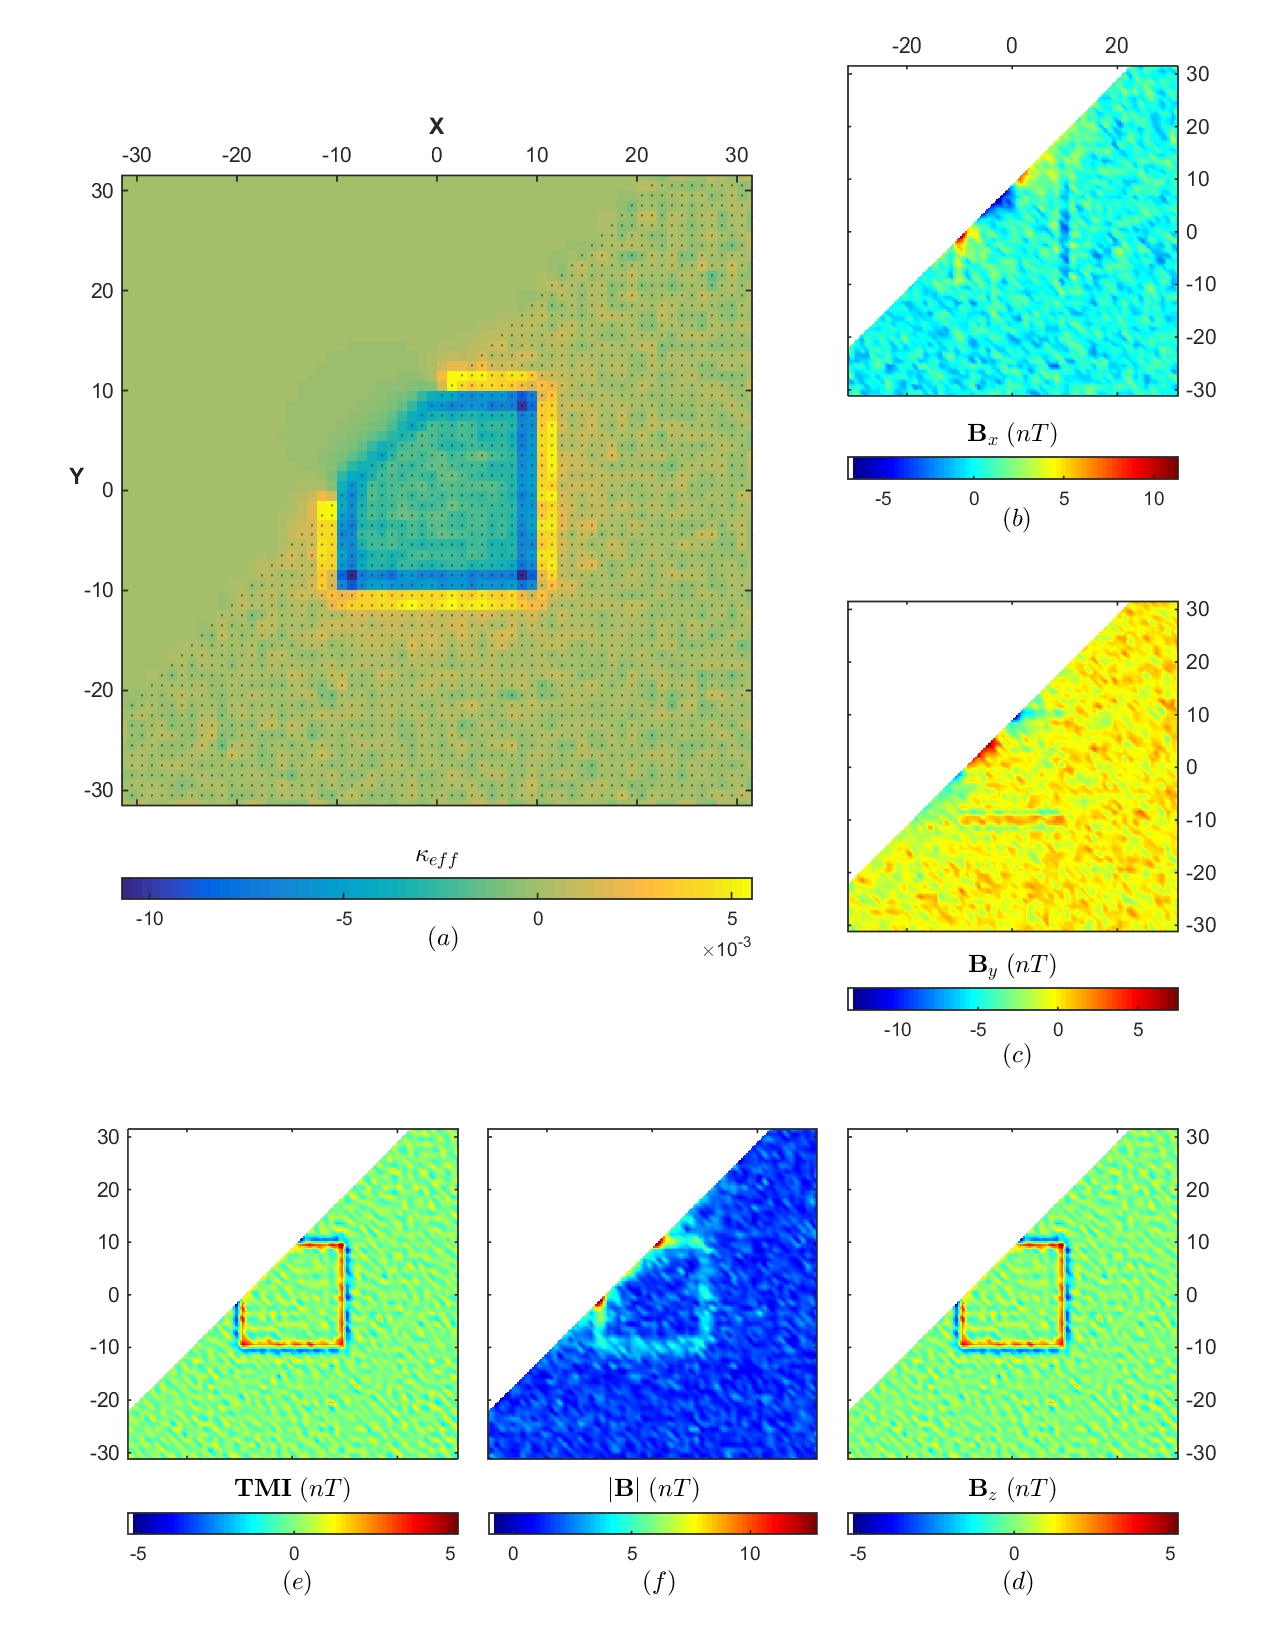
\includegraphics[scale=0.60]{EMS_CornerOut}
\caption{(a) Recovered Equivalent Magnetized Source (EMS) layer a subset of the original TMI data. The residual between observed and predicted data are shown in figure (b) to (f) for various components of the field. Structure in the $\hat x$ and  $\hat y$ components have been greatly reduced, yielding an amplitude data $\mathbf{|B|}$ with residual error within the uncertainty level of the noise.}
\label{fig:EMS_CornerOut}
\end{figure}

\section{Equivalent Magnitized Source Layer}

From experiment, I propose that the equivalent source needs to generate smooth field near the edge of the data in order to minimize such artefacts.
I propose an alternative equivalent source method that makes use semi-infinite prisms placed below the data. 
The benefit of using magnetized prisms is two folds. First, it speeds up data fitting as the algorithm can fit any orientation of magnetization and removes the assumtion that the filed is purely induced.
Secondly the method gives us an estimate of an effective magnetization direction, which can be fed as a warm start for the MAI and MVI inversion algorithms. This will prove to be important later.

Figure \ref{fig:EMS_CornerOut}

\endinput

